\documentclass[border=4pt]{standalone}
\usepackage{tikz}
\usetikzlibrary{arrows,arrows.spaced,positioning}
\begin{document}
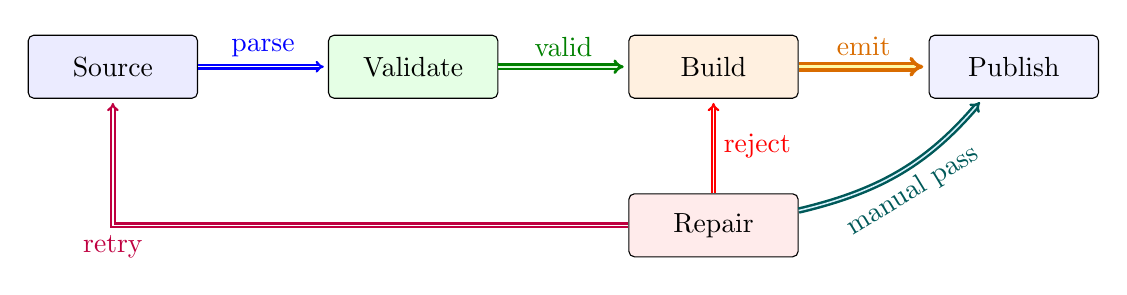
\begin{tikzpicture}[
  node distance=1.2cm and 1.65cm,
  stage/.style={draw,rounded corners=2pt,minimum width=2.15cm,minimum height=8mm,align=center}
]
  \node[stage,fill=blue!8] (source) {Source};
  \node[stage,fill=green!10,right=of source] (check) {Validate};
  \node[stage,fill=orange!12,right=of check] (build) {Build};
  \node[stage,fill=blue!6,right=of build] (ship) {Publish};
  \node[stage,fill=red!8,below=of build] (repair) {Repair};

  \draw[blue,double=white,line width=.8pt,double distance=.5pt,-{spaced implies}]
    (source) -- node[above]{parse} (check);
  \draw[green!50!black,double=green!12,line width=1pt,double distance=.6pt,-{spaced implies}]
    (check) -- node[above]{valid} (build);
  \draw[orange!85!black,double=yellow!35,line width=1.3pt,double distance=.9pt,-{spaced implies}]
    (build) -- node[above]{emit} (ship);
  \draw[red,double=white,line width=.8pt,double distance=.5pt,{spaced implies}-]
    (build) -- node[right]{reject} (repair);
  \draw[purple,double=white,line width=.8pt,double distance=.5pt,-{spaced implies}]
    (repair) -| node[below]{retry} (source);
  \draw[teal!70!black,double=cyan!16,line width=.9pt,double distance=.55pt,-{spaced implies}]
    (repair) to[bend right=18] node[below,sloped]{manual pass} (ship);
\end{tikzpicture}
\end{document}
